Let
\begin{align}
\vec{A}=\myvec{-3\\10},
\vec{B}=\myvec{6\\-8},
\vec{C}=\myvec{-1\\6}
\end{align}
Then by section formula,
\begin{align}
\vec{C}&=\frac{k\vec{B}+\vec{A}}{k+1}
\\
\myvec{-1\\6}&=\frac{1}{k+1}\myvec{6k-3\\-8k+10}
\\
\implies k&=\frac{2}{7}
\end{align}
The following Python code generates Fig. \ref{fig:3.6.3_section}
%
\begin{lstlisting}
solutions/3/codes/line/section/section.py
\end{lstlisting}
\begin{figure}[!ht]
\centering
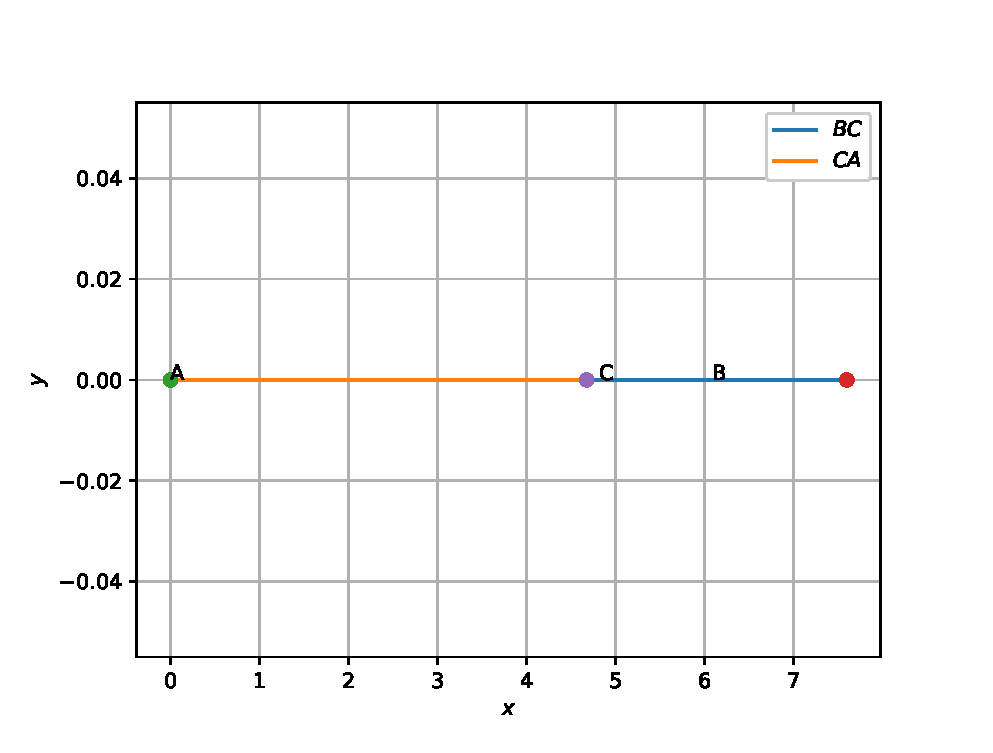
\includegraphics[width=\columnwidth]{./solutions/3/codes/line/section/pyfigs/section.eps}
\caption{C divides AB in ratio k:1}
\label{fig:3.6.3_section}
\end{figure}
